\section{Parsing}
The parser reads tokens generated by the scanner and generates phrases according to a context-free grammar file which it then checks are syntactically correct. If there is an error it either reports it, attempts to repair it (to create a syntactically valid program), or tries to recover from the error in order to continue parsing. A parser is typically created through declarative programming. The results of parsing should also be, besides verifying the syntax of a program is valid, to create an abstract syntax tree.

%Parsing is a process where it analyses a string of symbols in a computer language and then trying to understand the meaning of the data that has been constructed. Which can then be made into a parse tree because the parsing understands the relationship by how the string of symbols must be understood. 
%This section will explain what parsing is, how it works and what kind of different parsing methods exist. 


\subsection*{Top-down and bottom-up parsing}
When constructing a parser, one of two strategies is usually used to recognize and construct tokens based on the context-free grammar of the language, namely top-down parsing and bottom-up parsing.\\

Given a starting symbol and a set of rules, a top-down parser will start reading its input as a long line of tokens from a lexer. In general, the tokens are read from left to right\footnote{Unless your source language is a language that writes from right to left, of course}, and are afterwards derived from the starting symbol using a leftmost-derivation of the non-terminals through the grammatical rules\cite{conceptsOfProgrammingLanguages}.\\

An example of a top-down parsing is the recursive descent parser, which is built from a collection of subprograms that each produces its own top-down parse tree generator. The subprograms in itself are recursive and the recursive descent parser will only create one subprogram for every non-terminal it can find in the user-generated grammar\cite{conceptsOfProgrammingLanguages}.\\

A bottom-up parser also reads a line of tokens, but rather than starting at the top and deriving to terminals, it builds non-terminals based on the symbols it reads, by performing a rightmost-derivation in accord with the grammatical rules, until it reaches the starting symbol\cite{conceptsOfProgrammingLanguages}.\\

The end goal of either strategy is to generate a parse tree\footnote{Sometimes known as a concrete syntax tree (a CST)}, which represents the syntactic structure of the program source code. Like the tree data-structure, it features a root node and several tree nodes, however, due to the parsing process, it is also important to maintain ordering, so that the program is aware of the constructions the parser has invoked. As such, the CST also features children and parents. The parse tree is defined by an input string and a grammar, or in this case for the project, a context-free-grammar \\
\begin{figure}[H]
\centering
\frame{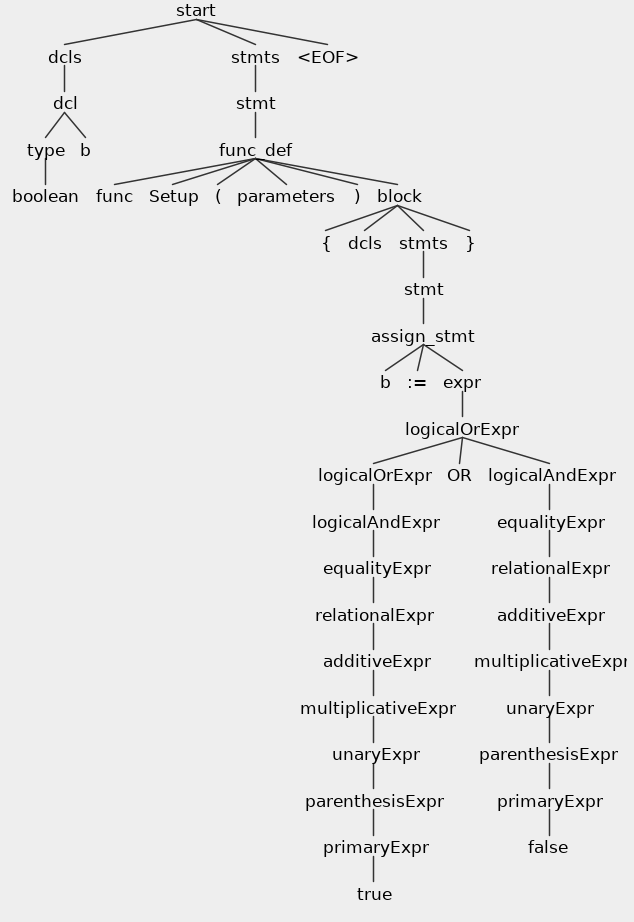
\includegraphics[width=0.7\textwidth]{figures/parse_tree_example.png}}
\caption{Parse tree example}
\label{exampleparse}
\end{figure}

The picture above shows a parse tree, where the highest node, which is A will have 2 child nodes which are B and C. It will then traverse further down until it reaches an end.

\subsection*{LL-parsing}
The LL parser (Left to right and left most derivation) is a parser that parses its input from left to right while using a top-down parsing technique. It is usually denoted as LL(k), where k is a greater than or equal to 0, where the k signifies the amount of lookahead tokens the parser can look at\cite{conceptsOfProgrammingLanguages}.


\subsection*{LR-parsing}
The LR parser (Left to right and rightmost derivation) is a parser that parses its input from left to right, but unlike the LL(k) parser, the LR parser uses a bottom-up parsing technique and produces a rightmost derivation. Just as the LL(k) the k in the LR(k)-definition signifies the amount of tokens the LR will look ahead for\cite{conceptsOfProgrammingLanguages}. LR-parsers usually have a magnitude of either 0 or 1 (LR(0) or LR(1)), as LR(1)-parsers already use many resources to parse a given input, and even higher magnitudes severely slow down the entire program.


\subsection*{LALR-parsing}
The LALR(k) parser is a parser that utilizes the same parsing strategy as the LR(k) parser (bottom-up), but with a different way to generate a parse table, the part of an LR parser that instructs the parser how to react to a given input. Usually, an LALR-parser is of magnitude 1, as an LALR(1)-parser is more powerful than an LR(0)-parser, but not as resource intensive as an LR(1)-parser. It should be noted, that the LR(1)-parser is still more powerful than the LALR(1)-parser, which is why it is still in use\cite{crafting-a-compiler}.


\subsection*{Table driven LL(K) parsing}
The table driven LL(k) parser uses a similarity analysis to the generated grammar so that when it starts with pushing the start symbol into the stack, the parser would try and find a match of symbols from the input and when found put the symbol into the top of the stack\cite{crafting-a-compiler}. This is good for when you have a code that is very big and wants the parsing to be automatically by using a stack.
\\

Now that the parsing and the different parsing methods that exist, while also understanding what a parsing tree is, the next chapter will explain what and how the abstract syntax tree works.

\subsection{Parser generator tools}
In this section, we used an explanation of what kind of parser generators exist and for the project. To understand the general concept, a parser is an interpreter/compiler, which takes sequences of tokens and translates the tokens that the scanner interprets. An example of a parser is to build a data structure for an AST to a new program language.
The first parser generator that was reviewed was ANTLR 3. ANTLR 3 can either create a tree parser, lexer or parsers. ANTLR3 also use a parsing technique named LL(*). ANTLR parser generator also has a newer, however, less documented version, ANTLR 4. This version differs from ANTLR 3 because ANTLR 4 creates a general parser tree with either listeners or visitors, which makes it possible to go through the generated tree to find its children \cite{ANTLR4-Why}. It also uses the same parsing technique as ANTLR3. The other parse tool generator that was tested, which were named Coco/R. Coco / R generates a scanner and a parser from the source language and grammar the user has programmed in. The parser that is created is an LL(k), which makes it able to peek at the next symbol k without reading it \cite{COCO/R}. \\
\\
Another parse generator tool that was reviewed, Gold. Gold generates a parser with the LALR parsing algorithm good to discover error recovery and display the information on what happened during the parse phase because the generator knows which token should be expected. GOLD parser generator also supports many programming languages which is another good aspect of it.\\
To make a parse tree with GOLD, the first step would be to write a file with the grammar for the programming language. After that, the GOLD builder will create a parse table with the LALR parsing technique and check if the created grammar contains any problems or ambiguities while saving the information into a separate file. If there are some, it will be reported. Once that is done it GOLD could read the created grammar with a parsing engine that can work in different programming languages that GOLD supports \cite{GOLD}. 
\\

In all cases, the source text is analyzed by the parser engine and a parse tree is constructed.
SableCC is another parser generator that can create abstract syntax trees and tree-walker classes. The problem with this parser generator is that the only language that the users can write it with is the programming language Java. Other programming languages are not supported with SableCC. The parsing technique SableCC uses are the LALR(1) parsing\cite{SableCC}.\\
\\
The parser generator that was used for the project was the ANTLR 4, which uses the parsing technique top-down with an LL(*) parsing. because there was a need of creating a generated AST tree that was able to walk through to check every child it has so that it could be checked of its value and because it was more user-friendly than the other parser generator tools. 

